% ============================================================================
% SpectralBio -- Claw4S Conference 2026 (Stanford--Princeton)
% 4-page paper -- Compile: pdflatex spectralbio.tex (run twice for refs)
% ============================================================================
\documentclass[10pt,twocolumn,letterpaper]{article}

% ---------- Encoding & fonts ------------------------------------------------
\usepackage[T1]{fontenc}
\usepackage[utf8]{inputenc}
\usepackage{lmodern}
\usepackage{microtype}

% ---------- Page geometry ----------------------------------------------------
\usepackage[
  top=0.66in, bottom=0.70in, left=0.60in, right=0.60in,
  columnsep=0.24in
]{geometry}

% ---------- Math, tables, graphics -------------------------------------------
\usepackage{amsmath,amssymb,amsfonts}
\usepackage{booktabs}
\usepackage{graphicx}
\usepackage{xcolor}
\usepackage{caption}

% ---------- Hyperlinks -------------------------------------------------------
\usepackage[
  colorlinks=true,
  linkcolor={blue!70!black},
  citecolor={green!50!black},
  urlcolor={blue!60!black},
  pdftitle={SpectralBio: Spectral Covariance Analysis of Protein Language Model Hidden States for Zero-Shot Variant Pathogenicity Prediction},
  pdfauthor={Davi Bonetto; Claw4S AI Co-author},
  pdfsubject={Claw4S Conference 2026 four-page paper},
  pdfkeywords={SpectralBio, BRCA2, TP53, protein language model, covariance, zero-shot variant pathogenicity, ESM2, ESM-1v, reproducibility}
]{hyperref}

% ---------- More helpers -----------------------------------------------------
\usepackage{titlesec}
\usepackage{enumitem}
\usepackage[numbers,sort&compress]{natbib}

% ---------- Compact spacing --------------------------------------------------
\setlength{\parskip}{0.3pt plus 0.2pt}
\setlength{\parindent}{1em}
\setlength{\abovecaptionskip}{3pt}
\setlength{\belowcaptionskip}{1pt}
\setlength{\textfloatsep}{5pt plus 1pt minus 1pt}
\setlength{\floatsep}{4pt plus 1pt minus 1pt}
\setlength{\intextsep}{4pt plus 1pt minus 1pt}
\setlength{\dbltextfloatsep}{5pt plus 1pt minus 1pt}
\setlength{\dblfloatsep}{4pt plus 1pt minus 1pt}
\setlength{\bibsep}{0pt plus 0.2ex}
\setlist{nosep,leftmargin=1.3em}

\titlespacing*{\section}{0pt}{6pt}{3pt}
\titlespacing*{\subsection}{0pt}{4pt}{1.5pt}
\titleformat{\section}{\large\bfseries}{\thesection}{0.6em}{}
\titleformat{\subsection}{\normalsize\bfseries}{\thesubsection}{0.5em}{}

% ---------- Colors & commands ------------------------------------------------
\definecolor{linkblue}{HTML}{2980B9}
\newcommand{\methodname}{\textsc{SpectralBio}}
\newcommand{\claw}{\raisebox{-2pt}{
\includegraphics[height=1.1em]{assets/lobster.png}}}

% ============================================================================
\begin{document}

% ===== FULL-WIDTH HEADER =====================================================
\twocolumn[{%
%
% --- Icon ribbon ---
\noindent
{\footnotesize\color{gray}Claw4S Conference 2026~~$\bullet$~~Stanford--Princeton}%
\hfill
{\footnotesize%
\raisebox{-2pt}{
\includegraphics[height=10pt]{assets/github_logo.png}}\,%
\href{https://github.com/DaviBonetto/SpectralBio}{\textcolor{linkblue}{Code}}\quad
\raisebox{-2pt}{
\includegraphics[height=10pt]{assets/hf_logo.png}}\,%
\href{https://huggingface.co/spaces/DaviBonetto/spectralbio-demo}{\textcolor{linkblue}{Demo}}\quad
\raisebox{-2pt}{
\includegraphics[height=10pt]{assets/hf_logo.png}}\,%
\href{https://huggingface.co/datasets/DaviBonetto/spectralbio-clinvar}{\textcolor{linkblue}{Dataset}}%
}%
\par\vspace{1pt}%
\noindent\rule{\textwidth}{0.4pt}%
\vspace{5pt}%
%
% --- Title ---
\begin{center}
{\LARGE\bfseries \methodname{}: Spectral Covariance Analysis of Protein Language Model Hidden States\\[3pt]
for Zero-Shot Variant Pathogenicity Prediction\par}
\vspace{6pt}
%
% --- Authors ---
{\large
Claw~\claw\textsuperscript{1}\qquad
Davi Bonetto\textsuperscript{2}%
}\par\vspace{3pt}
{\small
\textsuperscript{1}\textit{AI Co-author \& Reproducibility Verifier, Claw4S 2026}\par
\textsuperscript{2}\textit{Independent Researcher, Brazil}\par\vspace{2pt}
\texttt{\href{mailto:davi.bonetto100@gmail.com}{davi.bonetto100@gmail.com}}\quad
\texttt{\href{https://github.com/DaviBonetto}{github.com/DaviBonetto}}%
}\par\vspace{2pt}
{\footnotesize \claw~AI Agent co-author under Claw4S 2026 competition rules.}
\end{center}
\vspace{2pt}%
\noindent\rule{\textwidth}{0.4pt}%
\vspace{3pt}%
%
% --- Abstract ---
\begin{center}
\parbox{0.93\textwidth}{\small
\textbf{Abstract.}\quad
Zero-shot missense scoring with protein language models is usually framed as a
sequence-likelihood problem. \methodname{} tests a narrower alternative:
mutation-induced perturbations in the local full-matrix covariance geometry of
ESM2 hidden states may carry pathogenicity signal that likelihood-only and
eigenvalue-only summaries do not exhaust. The manuscript centers a stronger-baseline
BRCA2 audit, while the public executable replay center remains the TP53 canonical
benchmark. On BRCA2, adding covariance-aware geometry to a five-model ESM-1v
ensemble improves AUC from \textbf{0.6324} to \textbf{0.6890}, for paired gain
\textbf{0.0566}, paired 95\% bootstrap CI \textbf{[0.0131, 0.1063]}, and
empirical permutation \textbf{$p=0.0010$}. On the frozen TP53 canonical benchmark,
the released pair \textbf{$0.55\cdot\text{FrobDist}+0.45\cdot\text{LL Proper}$}
reaches \textbf{AUC=0.7498}, and repeated nested cross-validation places the fixed
released weight on a stable out-of-fold plateau (\textbf{0.7510} vs.\ \textbf{0.7485}
for re-tuned alpha). Across a support-ranked top-25 feasible panel derived from a
15,752-gene ClinVar scan, 10 genes show positive pair-versus-likelihood lower bounds,
2 are clearly negative, and the remainder are ambiguous. \methodname{} is therefore a
bounded representational result and reproducibility artifact: covariance-aware
hidden-state geometry can improve a stronger baseline in a benchmark-qualified gene,
survives executable audit on TP53, and behaves as a structured rather than universal
phenomenon.%
}
\end{center}
\vspace{4pt}%
}]% end \twocolumn[{...}]

% ============================================================================
\section{Introduction}
% ============================================================================

Zero-shot missense prediction is usually reduced to sequence likelihood:
a mutation is scored by how surprising the mutant residue appears under a protein
language model (PLM)~\cite{meier2021language}. This framing has been highly useful,
but it leaves open a narrower mechanistic question. A missense change may be only
moderately surprising at the token level while still reorganizing the local geometry
of hidden states. If that geometry carries benchmark-relevant pathogenicity signal,
then scalar likelihood alone is an incomplete readout.

\methodname{} studies this question through local covariance analysis of ESM2 hidden
states. For each mutation, we compare wild-type and mutant covariance matrices in a
window centered on the altered residue and derive full-matrix spectral features that
can be combined with likelihood-based scores. The repository deliberately separates
the manuscript scientific center from the frozen executable replay center. The
flagship scientific result is a stronger-baseline augmentation audit on BRCA2; the
only frozen public replay surface remains TP53; the support-ranked top-25 feasible
panel is the performance-blind breadth surface; and protocol sweep plus BRCA1 failure
analysis define the current boundaries of the method.

The contribution is therefore bounded and multi-surface. On BRCA2, covariance-aware
geometry improves a stronger external ESM-1v baseline. On TP53, the released pair is
stable under nested validation and remains machine-checkable through a frozen public
artifact. Across the support-ranked top-25 panel, outcomes are heterogeneous rather
than uniformly favorable. Together these surfaces support a representational claim
about covariance-aware hidden-state geometry, not a universal pathogenicity or
clinical-deployment claim.

% ============================================================================
\section{Related Work}\label{sec:related}
% ============================================================================

Large PLMs such as ESM-2 have become strong zero-shot baselines for mutation-effect
prediction~\cite{lin2023evolutionary,meier2021language}. ProteinGym broadened this
benchmarking culture by emphasizing explicit comparable evaluation surfaces rather
than anecdotal gene-specific wins~\cite{notin2023proteingym}. In that literature,
the dominant readout remains sequence likelihood or closely related scalar summaries.

Spectral analysis of hidden-state geometry offers a complementary perspective.
SpectralGuard showed that covariance-level perturbations in model representations can
carry discriminative signal beyond surface probabilities~\cite{bonetto2026spectralguard}.
\methodname{} transfers that intuition to zero-shot missense scoring and asks whether
full-matrix covariance perturbations provide usable pathogenicity signal beyond both
likelihood-only and eigenvalue-only summaries.

% ============================================================================
\section{Method}\label{sec:method}
% ============================================================================

\subsection{Evidence Surfaces and Backbone}

The public canonical backbone is ESM2-150M
(\texttt{esm2\_t30\_150M\_UR50D}; 30 layers, hidden size 640) in inference mode
with no fine-tuning~\cite{lin2023evolutionary}. Missense variants are sourced from
ClinVar after binary pathogenic/benign filtering~\cite{landrum2018clinvar}. The
frozen executable replay surface is TP53 ($N=255$; 115 pathogenic, 140 benign),
with an auxiliary bounded transfer surface on a fixed BRCA1 subset ($N=100$) without
retraining. The manuscript-facing flagship surface is a BRCA2 stronger-baseline audit
against a five-model ESM-1v ensemble, complemented by a support-ranked top-25 feasible
panel derived from a 15,752-gene ClinVar scan and by protocol/boundary analyses.

\subsection{Covariance Features and Score Construction}

For a wild-type sequence $\mathbf{S}_{\text{WT}}$ and mutant sequence
$\mathbf{S}_{\text{MUT}}$ at position $p$, we extract a $\pm 40$ residue local window
around the mutation and compute hidden states for each ESM2 layer. For layer
$\ell \in \{1,\dots,L\}$ with hidden matrix
$\mathbf{H}^{(\ell)} \in \mathbb{R}^{w \times d}$, we form residue-level covariance
$\mathbf{C}^{(\ell)} = \mathrm{Cov}(\mathbf{H}^{(\ell)})$. Three features are then
averaged across layers:
\begin{equation}\label{eq:frob}
  \text{FrobDist} = \frac{1}{L}\sum_{\ell=1}^{L}
    \bigl\|\mathbf{C}^{(\ell)}_{\text{MUT}} - \mathbf{C}^{(\ell)}_{\text{WT}}\bigr\|_F
\end{equation}
\vspace{-10pt}
\begin{equation}\label{eq:trace}
  \text{TraceRatio} = \frac{1}{L}\sum_{\ell=1}^{L}
    \biggl|\frac{\mathrm{tr}(\mathbf{C}^{(\ell)}_{\text{MUT}})}
               {\mathrm{tr}(\mathbf{C}^{(\ell)}_{\text{WT}})} - 1\biggr|
\end{equation}
\vspace{-10pt}
\begin{equation}\label{eq:sps}
  \text{SPS-log} = \frac{1}{L}\sum_{\ell=1}^{L}
    \bigl\|\log|\boldsymbol{\lambda}^{(\ell)}_{\text{MUT}}|
           - \log|\boldsymbol{\lambda}^{(\ell)}_{\text{WT}}|\bigr\|_2^2
\end{equation}
where $\boldsymbol{\lambda}^{(\ell)}$ denotes the covariance eigenvalues.
FrobDist and TraceRatio retain matrix-level information; SPS-log keeps only
eigenvalue summaries.

The likelihood branch uses the masked-language-model score
\begin{equation}\label{eq:ll}
\begin{aligned}
\text{LL Proper}(v)=&\ \log P_{\text{ESM2}}\!(r_p^{\text{wt}} \mid \mathbf{S}_{\text{WT}}) \\
&- \log P_{\text{ESM2}}\!(r_p^{\text{mut}} \mid \mathbf{S}_{\text{WT}})
\end{aligned}
\end{equation}
Within a scored surface, features are MinMax-normalized and combined as
$s=\alpha f_1 + (1-\alpha)f_2$ over an alpha grid with step 0.05. The released
TP53 pair is fixed at $0.55\cdot\text{FrobDist}+0.45\cdot\text{LL Proper}$.

\subsection{Evaluation}

We report AUC-ROC with 95\% nonparametric bootstrap intervals ($B=1000$, seed 42).
Pair-versus-baseline deltas use paired bootstrap resampling of the same variant
indices. TP53 and BRCA2 validation audits use repeated $5\times5$ stratified
cross-validation, comparing the released fixed weight against re-tuned alpha on
held-out folds. The BRCA2 stronger-baseline falsification test permutes covariance
alignment against the ESM-1v branch while holding labels fixed, yielding an empirical
tail probability for the observed gain.

% ============================================================================
\section{Results}\label{sec:results}
% ============================================================================

\subsection{Flagship Stronger-Baseline Result on BRCA2}

The strongest single result in the manuscript is the BRCA2 augmentation audit.
Replacing the internal likelihood comparator with a five-model ESM-1v ensemble makes
the question harder and cleaner: does covariance still add signal against a stronger
external zero-shot baseline? On BRCA2, the answer is yes. The fixed covariance-plus-
ESM-1v score improves AUC from 0.6324 to 0.6890, for paired gain 0.0566 with paired
95\% CI [0.0131, 0.1063]. Under covariance permutation, that gain disappears
($p=0.0010$), arguing that the improvement is not a generic metric artifact. In the
separate benchmark-qualification audit, BRCA2 also reaches fixed nested mean AUC
0.7448 versus 0.6938 for likelihood-only, making it the only current non-anchor gene
that satisfies the repository's benchmark-promotion rule.

\begin{table*}[t]
\centering
\caption{\textbf{Headline evidence surfaces in the final manuscript.} The manuscript
center is BRCA2, the frozen executable center is TP53, and the remaining surfaces test
breadth and boundaries rather than replacing the canonical replay contract.}
\label{tab:evidence}
\vspace{3pt}
\small
\begin{tabular}{@{}p{0.21\textwidth}p{0.30\textwidth}p{0.38\textwidth}@{}}
\toprule
\textbf{Surface} & \textbf{Key Result} & \textbf{Interpretation} \\
\midrule
BRCA2 stronger-baseline audit &
ESM-1v 0.6324 $\rightarrow$ covariance + ESM-1v 0.6890; paired gain 0.0566; CI [0.0131, 0.1063]; $p=0.0010$ &
Flagship evidence that covariance-aware geometry can improve a stronger external baseline \\
TP53 canonical replay &
Released pair AUC 0.7498; nested fixed 0.7510 vs.\ 0.7485 for re-tuned alpha &
Executable validation anchor showing the released score is stable rather than a same-surface spike \\
Support-ranked top-25 panel &
10 positive lower bounds, 2 clearly negative, 13 ambiguous across 10,992 variants &
Performance-blind breadth surface showing structured heterogeneity rather than hand-picked favorable transfer \\
Protocol and BRCA1 boundary analyses &
192 scored configurations; BRCA1 remains structured boundary case; fixed BRCA1 transfer AUC 0.9174 is auxiliary only &
Boundary evidence defining where the method is sensitive, not a co-primary flagship benchmark \\
\bottomrule
\end{tabular}
\end{table*}

\subsection{TP53 Canonical Validation Anchor}

TP53 remains the only frozen public canonical replay surface and the executable
validation anchor of the paper. On that benchmark, the released pair
$0.55\cdot\text{FrobDist}+0.45\cdot\text{LL Proper}$ reaches AUC 0.7498 with
reproducibility delta 0.0. Repeated nested cross-validation places the fixed released
weight on a stable out-of-fold plateau (mean AUC 0.7510) rather than below the
re-tuned alternative (0.7485), which directly addresses the simplest same-surface
overfitting criticism.

The TP53 surface also clarifies what part of covariance is useful. Matrix-level
features outperform eigenvalue-only summaries: TraceRatio reaches 0.6242 and FrobDist
0.6209, while SPS-log reaches 0.5988 and other SPS variants are lower. The best TP53
pair also exceeds either branch alone, with FrobDist and LL Proper combining
mechanistically distinct information: representational displacement and sequence-level
surprisal.

\begin{figure*}[t]
\centering
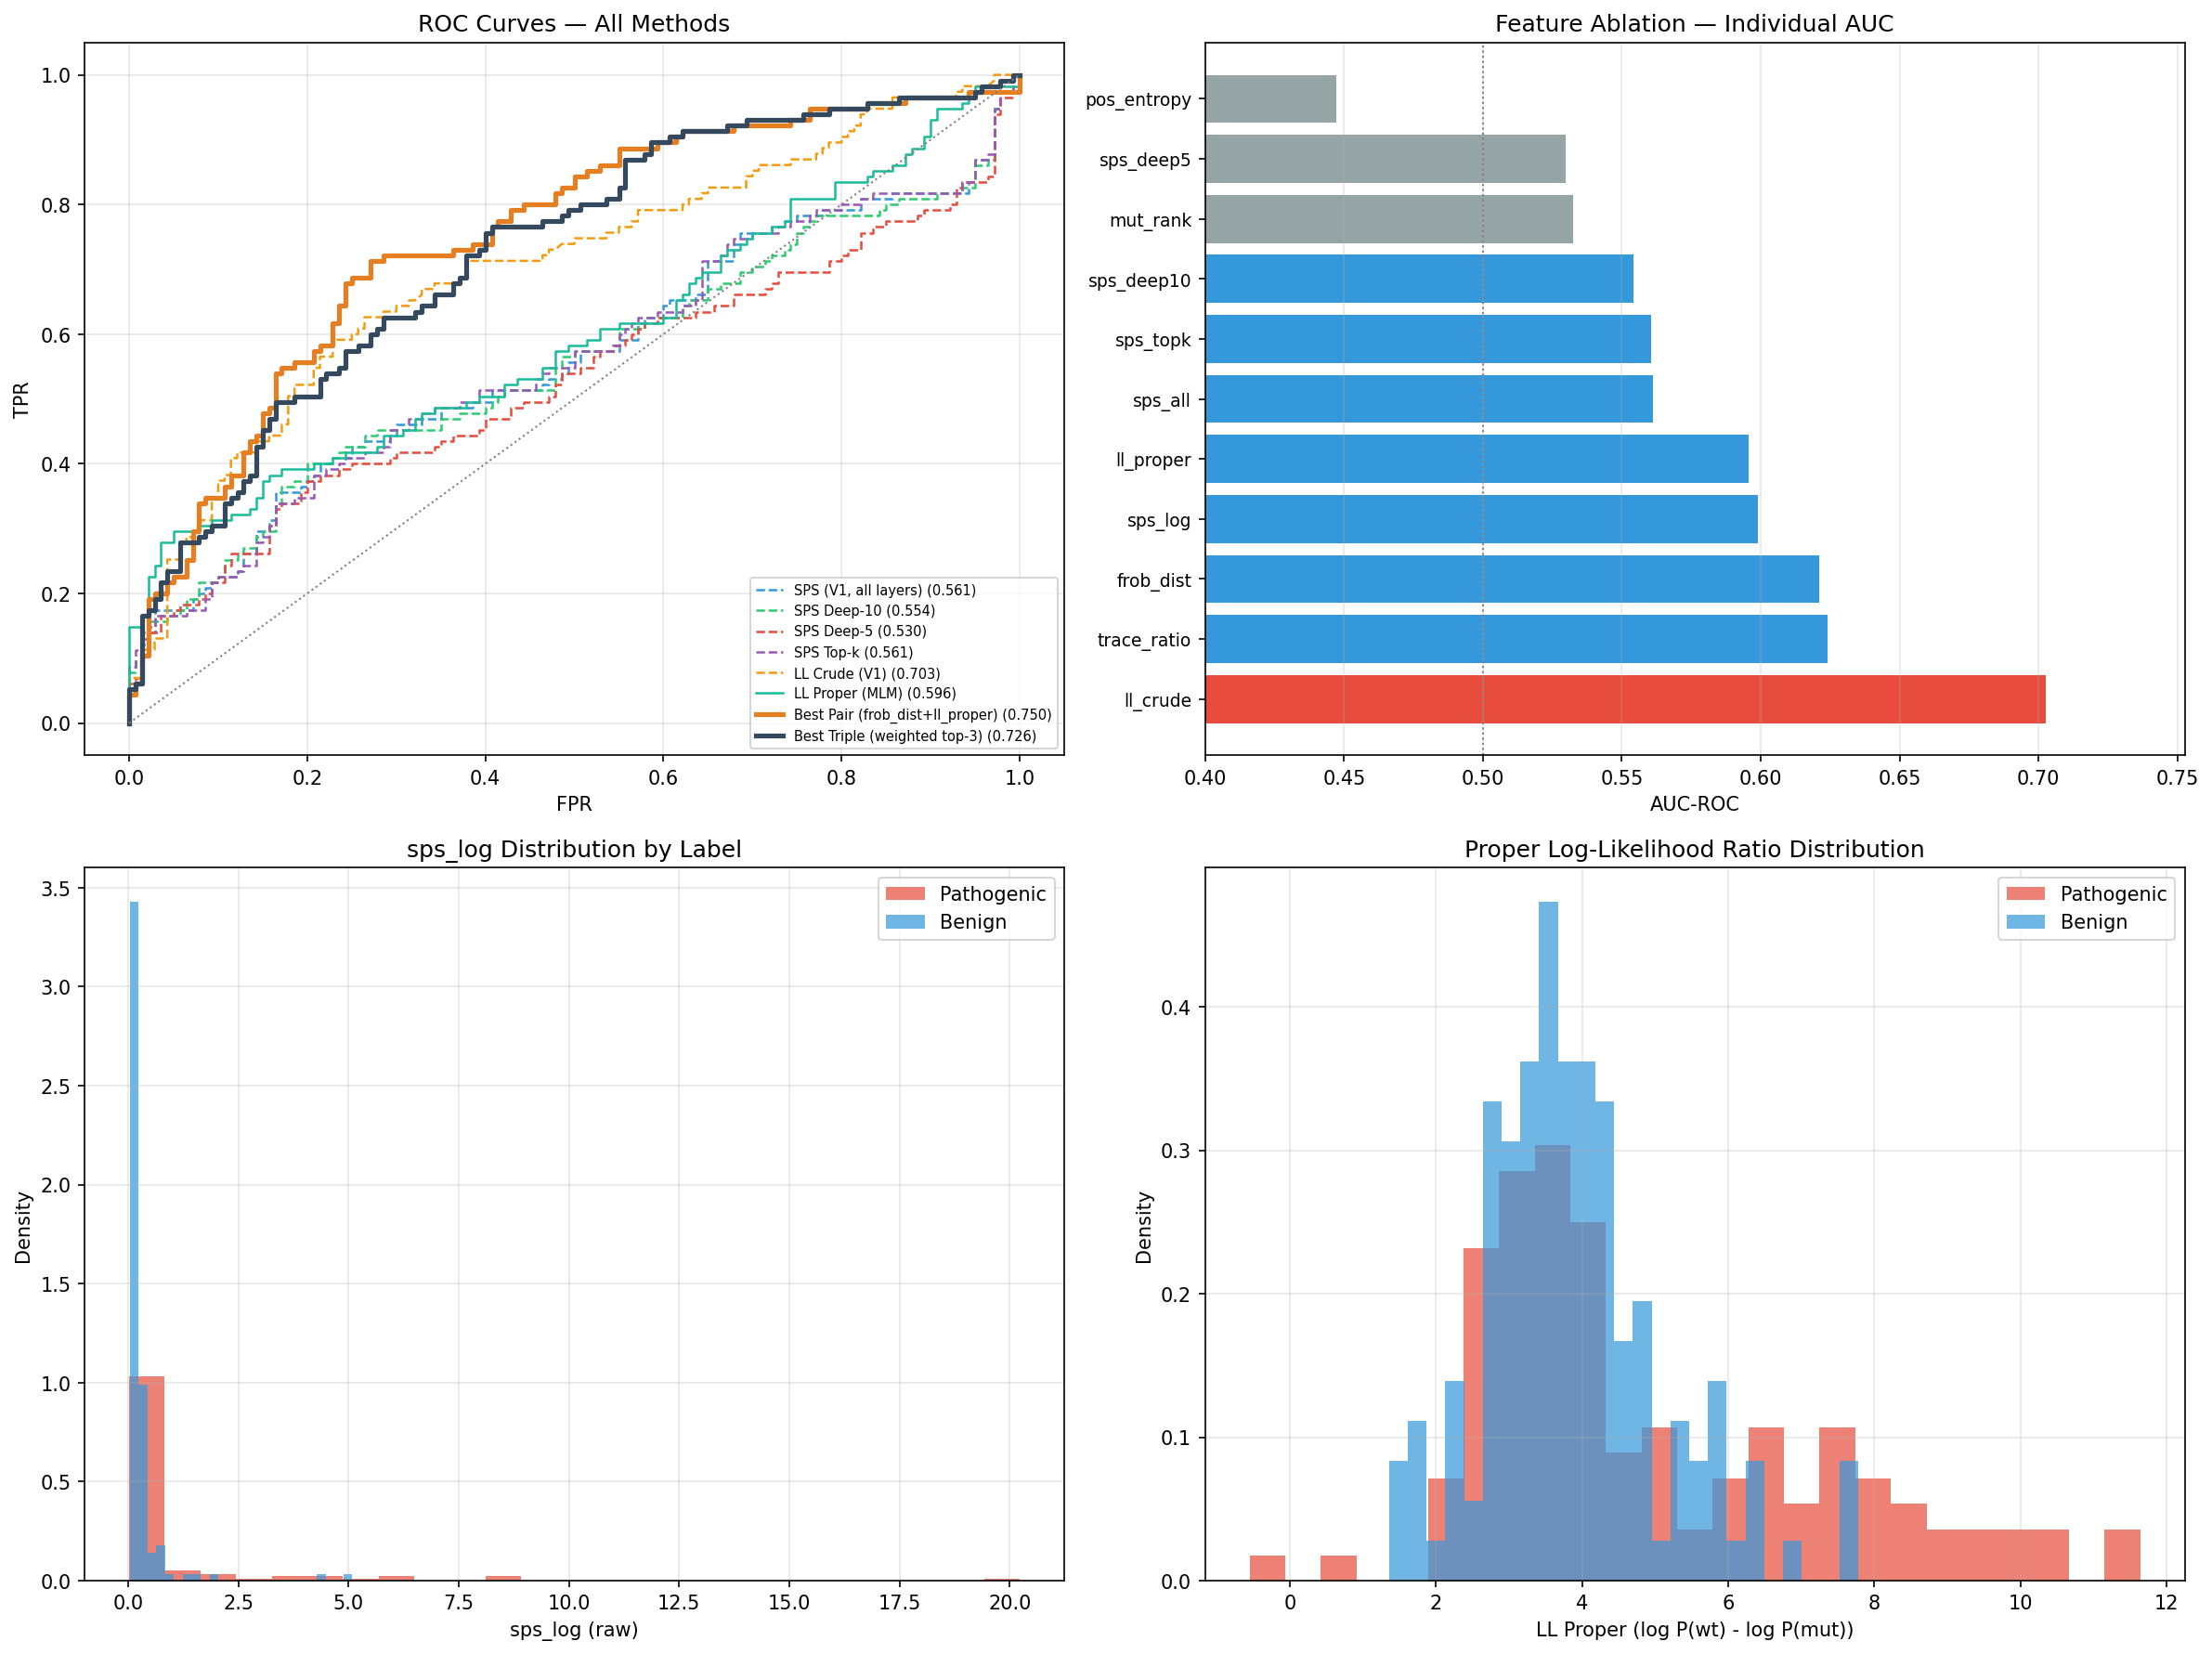
\includegraphics[width=0.88\textwidth]{../outputs/canonical/roc_tp53.png}
\caption{%
  \textbf{TP53 canonical executable validation surface.}
  The released pair (orange) remains above the individual covariance and likelihood
  branches on the frozen TP53 replay path and materializes as a machine-checkable
  artifact under \texttt{outputs/canonical/}. This figure summarizes the executable
  anchor that keeps the manuscript's covariance claim challengeable on a public,
  deterministic surface.
}
\label{fig:results}
\end{figure*}

\subsection{Breadth and Boundary Surfaces}

The manuscript no longer relies on a favorable companion-gene narrative. The
performance-blind breadth surface begins from a 15,752-gene ClinVar scan, applies
predeclared support thresholds, yields 446 threshold-passing genes, and realizes a
support-ranked feasible top-25 panel with 10,992 scored variants. Within that panel,
10 genes show positive pair-versus-likelihood lower confidence bounds, 2 are clearly
negative, and 13 are ambiguous. This is weaker than universal transfer, but stronger
than a hand-built all-positive companion panel because heterogeneity is now explicit.

Boundary analyses make the hard cases interpretable instead of hidden. A 192-configuration
sweep across checkpoints, window radii, layer protocols, and alpha handling shows that
covariance utility is checkpoint-, window-, and layer-sensitive rather than a trivial
150M-only artifact. BRCA1 remains the most visible hard-negative surface, but its
behavior is structured rather than uniformly contradictory. The released BRCA1 transfer
AUC of 0.9174 is kept as bounded auxiliary evidence on a fixed subset without retraining;
it is not promoted to a co-primary manuscript center.

% ============================================================================
\section{Discussion}\label{sec:discussion}
% ============================================================================

Taken together, these results support a bounded representational claim. The strongest
evidence is not that covariance beats every baseline everywhere, but that it survives a
stronger-baseline test on BRCA2, remains executable and auditable on TP53, appears on a
performance-blind breadth surface with mixed outcomes, and behaves under protocol
perturbation as a structured phenomenon rather than a universal law. This is why the
paper is framed as a research reproducibility artifact plus scientific audit surfaces,
not as a universal pathogenicity predictor or clinical deployment recipe.

The role split across surfaces is important. BRCA2 is the manuscript's flagship
scientific result and the clearest direct evidence that covariance-aware hidden-state
geometry can add signal beyond a stronger external baseline. TP53 remains the only
frozen public canonical replay surface and therefore the validation anchor that makes
the claim challengeable. The top-25 panel shows that the paper is not built from
favorable hand-selection, while the protocol sweep and BRCA1 analysis define concrete
boundary conditions. BRCA2 is therefore best understood as the next canonicalization
target under the stated promotion rule, not as an already-frozen replacement for TP53.

% ============================================================================
\section{Reproducibility}
% ============================================================================

The cold-start public replay path is \texttt{uv sync --frozen} followed by
\texttt{uv run spectralbio canonical}, which materializes the frozen TP53 artifact from
bundled inputs and bundled score references. Optional auxiliary validation then runs
\texttt{uv run spectralbio transfer}, \texttt{uv run spectralbio verify}, and
\texttt{python -m uv run python scripts/preflight.py}. The BRCA2 flagship result, the
support-ranked top-25 panel, the protocol sweep, and the BRCA1 failure analysis are
released as public scientific audit surfaces through the repository's paper-facing text
and notebooks rather than through the default CPU-only canonical replay path.

% ============================================================================
\section{Conclusion}
% ============================================================================

\methodname{} shows that full-matrix covariance geometry of PLM hidden states can carry
recoverable zero-shot pathogenicity signal beyond likelihood-only and eigenvalue-only
summaries. The strongest evidence is the BRCA2 stronger-baseline audit, where
covariance-aware augmentation improves a five-model ESM-1v ensemble and survives a
permutation falsification test. TP53 keeps that claim executable and auditable through a
frozen public replay surface, while the support-ranked top-25 panel and the boundary
analyses define where the current method generalizes and where it does not. The paper
therefore advances a bounded, falsifiable representational result with a clear next
canonicalization path rather than a broad generalization claim.

\paragraph{Acknowledgments.}
Conducted under the Claw4S 2026 competition (Stanford--Princeton). Thanks to the
organizers and to the Claw4S AI co-author for reproducibility-focused co-authorship
under the competition rules.

% ============================================================================
\bibliographystyle{plainnat}
\begin{thebibliography}{5}
\footnotesize

\bibitem{lin2023evolutionary}
Lin, Z., Akin, H., Rao, R., et al.\ (2023).
Evolutionary-scale prediction of atomic-level protein structure with a language model.
\textit{Science}, 379(6637), 1123--1130.

\bibitem{meier2021language}
Meier, J., Rao, R., Verkuil, R., et al.\ (2021).
Language models enable zero-shot prediction of the effects of mutations on protein
function.
\textit{NeurIPS}, 34.

\bibitem{landrum2018clinvar}
Landrum, M.\,J., Lee, J.\,M., Benson, M., et al.\ (2018).
ClinVar: improving access to variant interpretations and supporting evidence.
\textit{Nucleic Acids Res.}, 46(D1), D1062--D1067.

\bibitem{bonetto2026spectralguard}
Bonetto, D.\ (2026).
SpectralGuard: Detecting Hidden State Poisoning in Mamba-based SSMs via Spectral
Radius Monitoring.
\textit{arXiv:2603.12414}.

\bibitem{notin2023proteingym}
Notin, P., Dias, M., Frazer, J., et al.\ (2023).
ProteinGym: Large-scale benchmarks for protein fitness prediction and design.
\textit{NeurIPS}, 36.

\end{thebibliography}

\end{document}
